\section{Task 6: From Light Blond to Black}
\label{sec:task6}

\subsection{Results for All Beer Colours}
\label{sec:task6-results}
The full quality-constrained model from Task 5 is solved for each colour class. Black beer is modelled as $\EBC \geq 120+\epsilon_{\EBC}$, with $\epsilon_{\EBC}=10^{-6}$, because the assignment specifies $\EBC>120$.

\begin{table}[H]
\renewcommand{\arraystretch}{1.15}
\caption{Task 6 Results for All Beer Colours}
\label{tab:task36-colors}
\centering
\small
\begin{tabular}{@{}llrlrp{0.24\textwidth}@{}}
\toprule
Colour & EBC range & Feasible & Cost & Achieved EBC & Notes \\
\midrule
light blond & 6--8 & no & -- & -- & No feasible quality-constrained mix found. \\
blond & 9--12 & yes & 4919.601 & 12.000 & Uses the upper blond boundary. \\
gold & 13--19 & yes & 4883.000 & 14.535 & Cheapest feasible colour in this run. \\
amber & 20--29 & yes & 4891.923 & 20.000 & Same setup as Task 5. \\
copper & 30--45 & yes & 4908.251 & 30.000 & Uses the lower colour boundary. \\
brown & 46--75 & yes & 4934.376 & 46.000 & Darker colour requires a different source mix. \\
dark brown & 76--120 & yes & 4983.359 & 76.000 & Upper bound remains 120. \\
black & $>120$ & yes & 5061.830 & 120.000001 & Modelled as $120+\epsilon_{\EBC}$. \\
\bottomrule
\end{tabular}
\end{table}

Table~\ref{tab:task36-solution-summary} gives the selected process choice and achieved qualities for each feasible colour. Table~\ref{tab:task36-nonzero-ingredients} gives the corresponding non-zero ingredient mixes.

\begin{table}[H]
\renewcommand{\arraystretch}{1.15}
\caption{Task 6 Solution Summary for Feasible Beer Colours}
\label{tab:task36-solution-summary}
\centering
\small
\begin{tabular}{@{}lcrrrrr@{}}
\toprule
Colour & Process & Cost & EBC & $Q_S$ & $Q_H$ & $Q_Y$ \\
\midrule
blond & $(0,1)$ & 4919.601 & 12.000 & 3.000 & 3.000 & 3.000 \\
gold & $(0,1)$ & 4883.000 & 14.535 & 3.000 & 3.000 & 3.000 \\
amber & $(0,1)$ & 4891.923 & 20.000 & 3.000 & 3.000 & 3.000 \\
copper & $(0,1)$ & 4908.251 & 30.000 & 3.000 & 3.000 & 3.000 \\
brown & $(0,1)$ & 4934.376 & 46.000 & 3.000 & 3.000 & 3.000 \\
dark brown & $(0,1)$ & 4983.359 & 76.000 & 3.000 & 3.000 & 3.000 \\
black & $(0,1)$ & 5061.830 & 120.000001 & 3.000 & 3.000 & 3.000 \\
\bottomrule
\end{tabular}
\end{table}


\begin{table}[H]
\renewcommand{\arraystretch}{1.12}
\caption{Task 6 Non-Zero Ingredient Mixes for Feasible Colours}
\label{tab:task36-nonzero-ingredients}
\centering
\scriptsize
\begin{tabular}{@{}lp{0.78\textwidth}@{}}
\toprule
Colour & Non-zero ingredients \\
\midrule
blond & malt03 454.842 kg; malt04 332.737 kg; malt11 166.368 kg; hop07 3.421 kg; hop10 3.421 kg; yeast03 3.750 kg \\
gold & malt03 953.947 kg; hop07 3.421 kg; hop10 3.421 kg; yeast03 3.750 kg \\
amber & malt03 901.457 kg; malt06 17.497 kg; malt12 34.994 kg; hop07 3.421 kg; hop10 3.421 kg; yeast03 3.750 kg \\
copper & malt03 805.411 kg; malt06 49.512 kg; malt12 99.024 kg; hop07 3.421 kg; hop10 3.421 kg; yeast03 3.750 kg \\
brown & malt03 651.737 kg; malt06 100.737 kg; malt12 201.474 kg; hop07 3.421 kg; hop10 3.421 kg; yeast03 3.750 kg \\
dark brown & malt03 363.598 kg; malt06 196.783 kg; malt12 393.566 kg; hop07 3.421 kg; hop10 3.421 kg; yeast03 3.750 kg \\
black & malt01 72.431 kg; malt06 293.839 kg; malt12 587.677 kg; hop07 3.421 kg; hop10 3.421 kg; yeast03 3.750 kg \\
\bottomrule
\end{tabular}
\end{table}


\subsection{Cost as a Function of Beer Colour}
\label{sec:task6-plot}
The minimum cost for each feasible colour is plotted in Figure~\ref{fig:task36-cost-color}.

\begin{figure}[H]
\centering
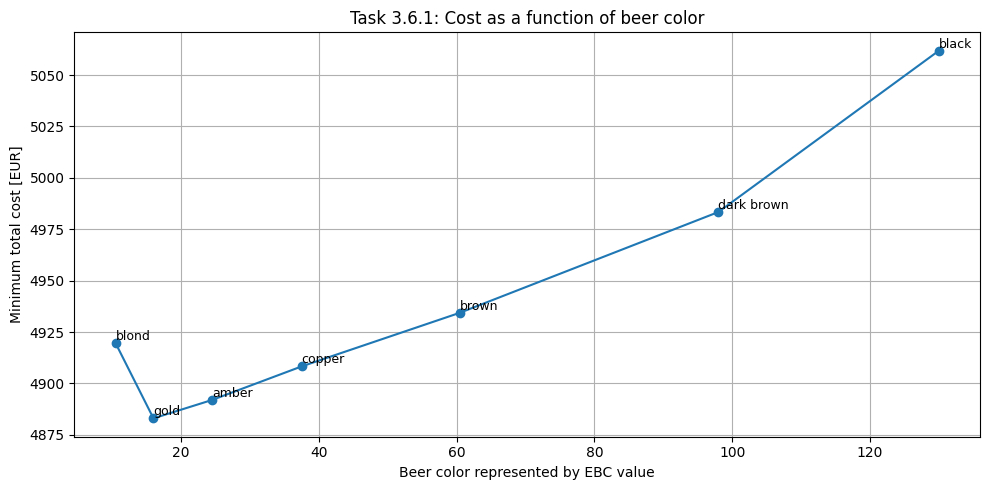
\includegraphics[width=\linewidth]{bilder/task_36_cost_by_color.png}
\caption{Task 6 minimum production cost for each feasible beer colour.}
\label{fig:task36-cost-color}
\end{figure}

\subsection{Explanation}
\label{sec:task6-explanation}

The cost differences are caused by the available EBC values and quality scores in the dataset. Gold is the cheapest feasible colour in Table~\ref{tab:task36-colors}, while black is the most expensive feasible colour. All feasible colour classes use the same process choice, $(0,1)$, so the main cost change comes from the fermentable-source mix rather than from different fixed process costs.

Light blond is infeasible because no available quality-constrained weighted EBC mix satisfies the low EBC interval 6--8. As the required colour becomes darker, the model introduces darker and more expensive malt sources to move the weighted EBC average upward. Black is feasible only by reaching just above the strict 120 EBC boundary, represented in the LP as $120+\epsilon_{\EBC}$.
% Values in this section come from the updated task_36.ipynb after the black EBC epsilon fix.
